% !TEX root = ./main.tex

\textbf{Results}

\textbf{Complementary Transitions Implies Hydrophobic Effect}

How do MSMs from solvent coordinates match up with the protein centric
view? Solvent and protein transitions are found to be interconnected,
such that when mapping each set of input features to the first two
slowest-relaxing components there exists overwhelming similarities.
Furthermore, potential energy wells overlap for the two largest tICA
components, tIC1 and tIC2. Also, the metastable states that correspond
to these basins are identical for both tICA landscapes. Many have
proposed various roles for water molecules, such as water enslaving
protein motions (2). Here, in fine detail the latter proposal was
scrutinized by exposing the solvent shells that contributed to the
slowest motions in the de-wetting process and emphasizing the
consequence of solvent density within the binding site.

Previously, analysis of protein centric viewpoint of binding has been
performed. Reconstruction of this protein centric MSM as well as the
investigation of the role of water by constructing an MSM using solvent
features enables a side-by-side (Figure S1.) comparison of the two tICA
landscapes. The first used protein pair distances and the other solvent
shell features metric, where each contained equivalent model parameters.
Remarkably, by scoping into the solvent map at each of the corners, the
four main states based on reaction coordinates are also found at these
exact locations as well as all other locations. Our tICA map using
solvent shell features reveals that the four main states are as follows
(figure 3.): top left represents the unbound-unfolded, bound-unfolded in
the top right, bound-folded in the bottom right, bottom left is the
bound-unfolded.

That's not all, the correlation with Tryptophan, W23 of p53, and tIC2
still exists in the solvent MSM. It has been found that trajectories
that come from (+tIC1, +tIC2), and finish at the native state in the
bottom right predominantly display W23 facing out of the page when
looking at MDM2-p53 from the orientation shown in all the figures from
this work. On the contrary, when W23 is oriented into the page for
trajectories mapped to the region with -tIC1 and -tIC2 (refer to Fig.
5). An observed trend, post binding of MDM2-p53, there exists water
association in the pocket and many of the trajectories require an
increase of water fluctuation to induce burrowing of W23.

The second tICA component relates to the first component, which can be
described as de-wetting. When moving from -tIC1 to +tIC1, there is a
direct correlation to the number of water molecules inside the pocket,
which corresponds to how close p53 is to MDM2's binding site. Hence the
location of the native state residing in the lower right corner (+tIC1,
-tIC2). When bulky residues enter the hydrophobic pocket, water tends to
relocate to find more polar interactions. For example, as W23 enters the
pocket with or without the correct orientation, there is a shift along
the trajectory to a more positive tIC1 value. Stability of the bound
alpha helix is maximized when W23 is in the correct orientation (into
page). Furthermore, when F19 also buries deep inside the cleft there is
a significant shift along tIC1 regardless of W23's orientation (+tIC1,
±tIC2).

\textbf{Slowest-dyanmical Solvent Features}

Solvent shell featurization achieves instantaneous solvent density with
respect to solvent features over all trajectories (9). Solvent features
are determined by the binning of water molecules when considering only
solute-solvent distances. The alpha and beta carbons as in the
previously tested protein pair distance metric were used, where each of
the 63 solute atoms contained 4 equidistant shells around them for a
total of 252 solvent features. Fitting the feature vector containing
every trajectory to the tICA model, which produced a linear combination
of water features. After construction of the 10-component tICA model,
which serves as the new basis set for the data, we subsequently built a
solvent MSM following equivalent parameters as Zhou et al.

Information about each individual solvent feature that correlate to the
slowest-dynamical motions of de-wetting was then extracted after
applying the 1\textsuperscript{st} component. From this, an overall
determination of water flux is found (Fig 3.). The degree of
contribution the slowest dynamical motions within a specific shell (Fig.
3) are taken from the coefficients of the normalized
1\textsuperscript{st} eigenvector squared. To obtain the magnitude of
significance while eluding from noise, the coefficients of the applied
eigenvector were squared and divided by the magnitude of the applied
eigenvector, hence the normalized 1\textsuperscript{st} eigenvector
squared.

The residues contributing to the slowest motions are extracted from the
normalized first eigenvector squared (Fig. 3) and can be seen when
looking at Figure 2. below. The slow-dynamical solvent features included
the first shell (0-3 Å) of Histidine, H73 (α) and Glutamine, Q72 (α, β)
of MDM2 along with the second shell (3-6 Å) of K24(α, β) and T18(α, β)
of p53 as the features contributing to the slowest motions involved in
de-wetting. The flux of solvent dynamics of these specific solute atoms
are colored according to a solvation gradient, where pink represents an
inward flux, orange is neutral, and yellow an outward flux.

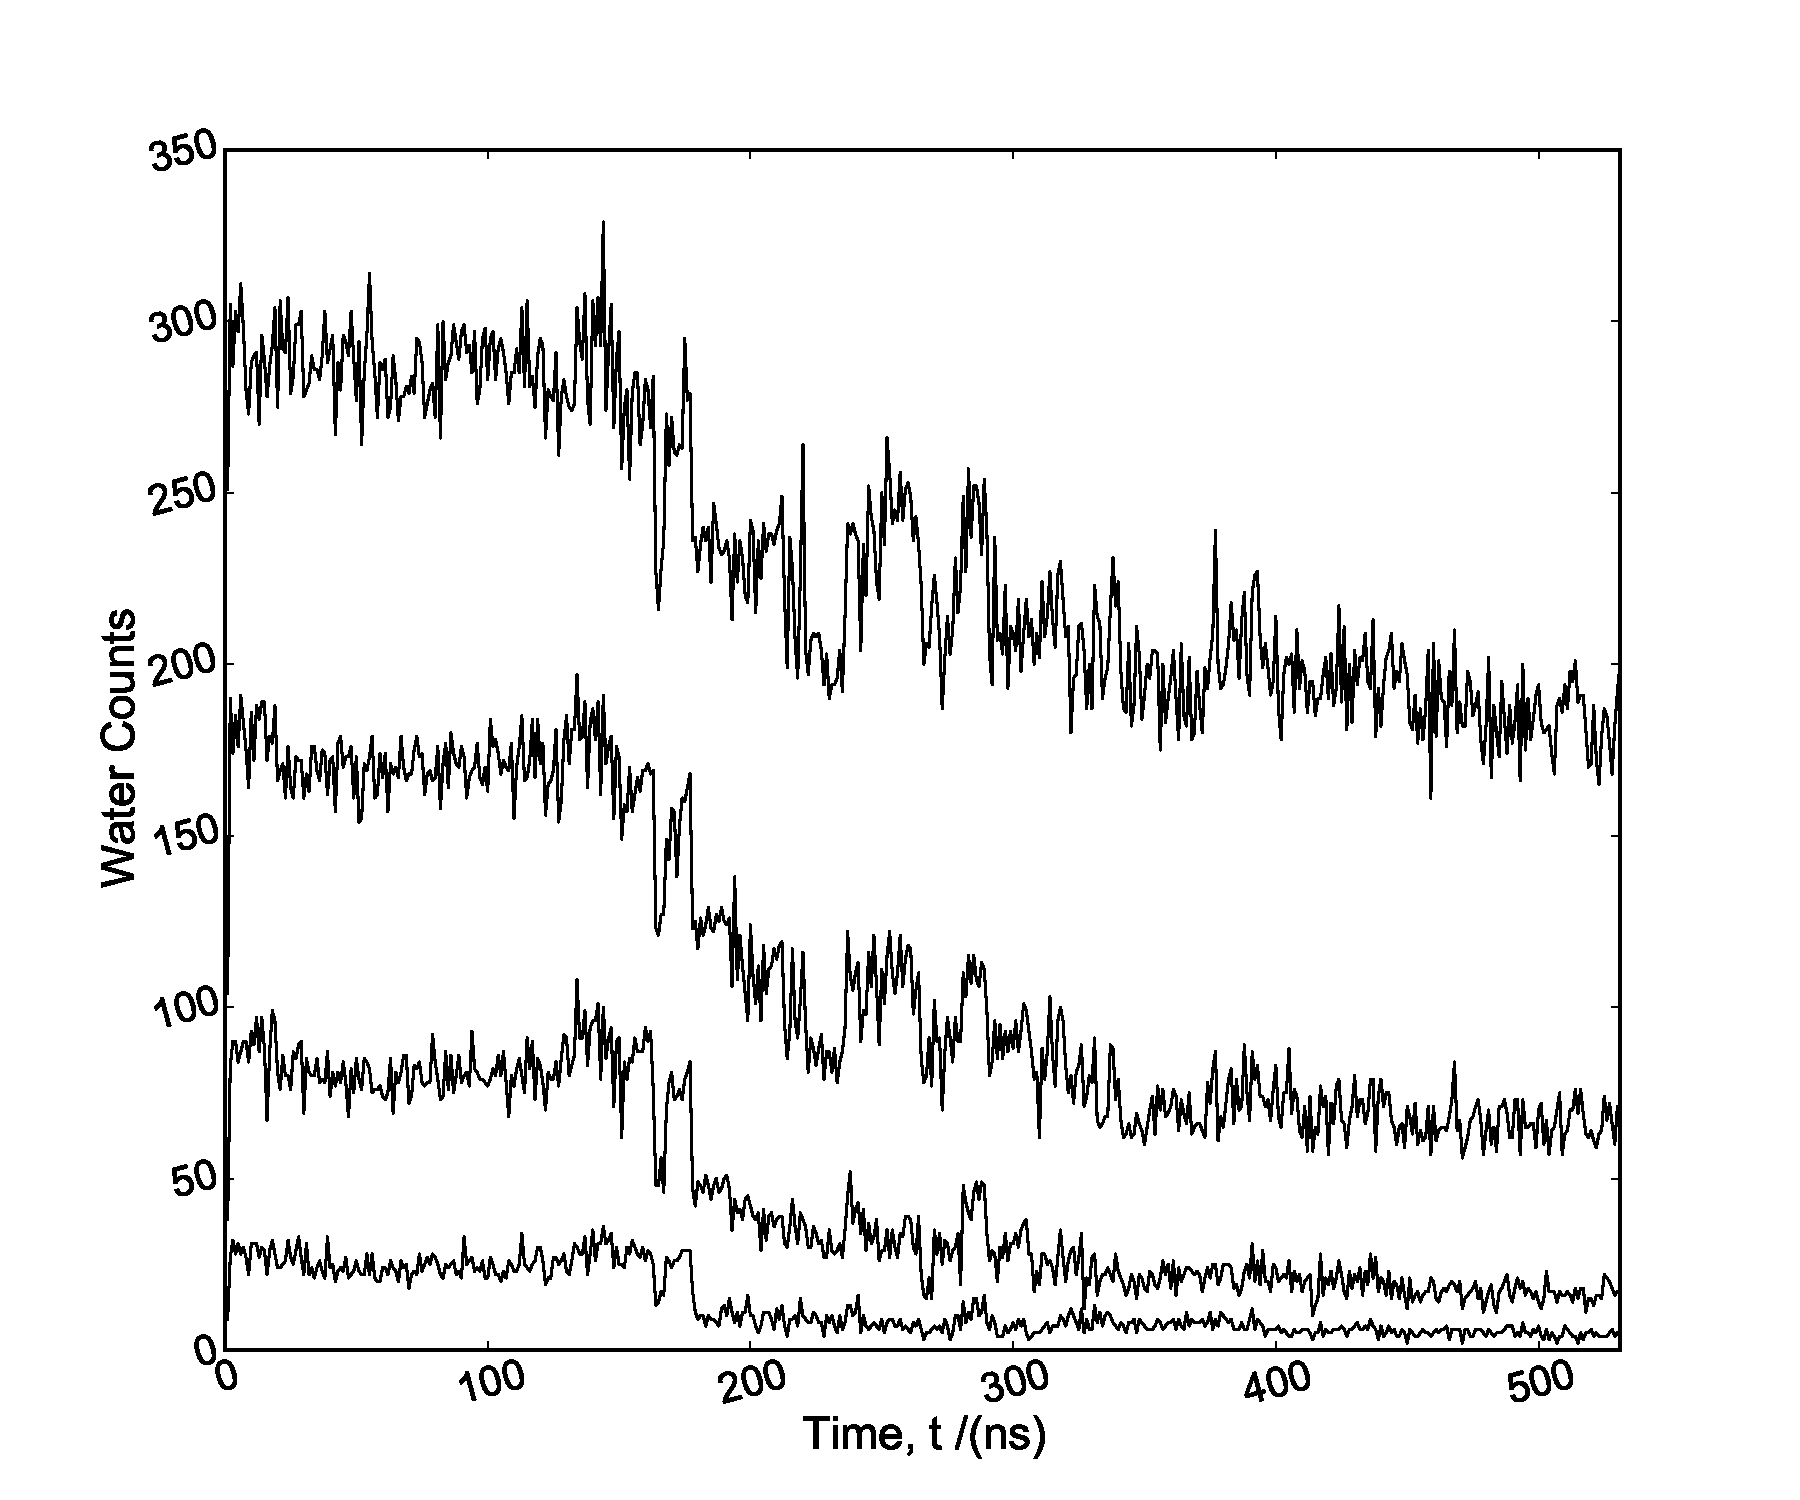
\includegraphics[width=4.73in,height=4in]{media/image2.emf}

\textbf{Figure 2.} MDM2 (blue) and p53 (green)~shown with residues
(silver, orange, pink, and yellow) containing Cα and Cβ solute atoms
selected for water shell featurization. Significant residues are
identified from the normalized squared components of the
1\textsuperscript{st} eigenvector (see Fig. 3) and colored accordingly.

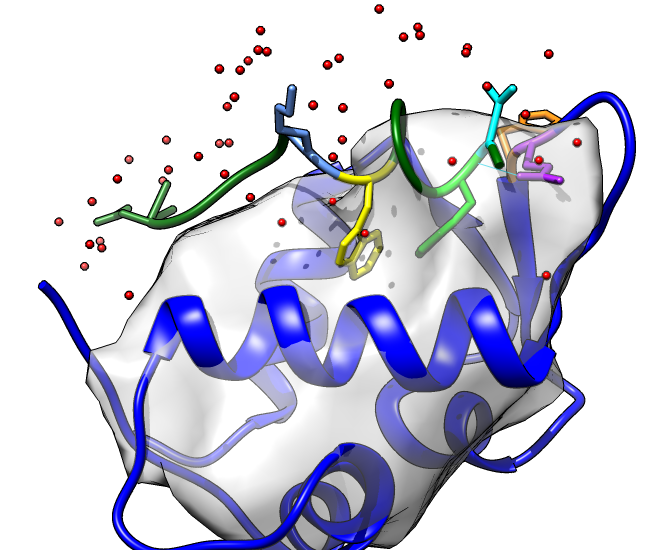
\includegraphics[width=6.5in,height=5.41944in]{media/image3.emf}

\textbf{Figure 3.} \textbf{Solvent shells around key residues contribute
to the slowest de-wetting motions.} (Top) The degree of contribution for
each solvent shell. Significant slow-dynamical solvent features are
labeled by carbon atom and residue to which it belongs. The green and
blue slices denote groups of residues for p53 and MDM2, respectively.~
(Bottom) The flux of significant solvent dynamics relative to distinct
solvent shells are represented by pink (solvation) and yellow dots
(de-wetting).

Information regarding specific shells must be taken from the
eigenvector, which requires decomposition to investigate each of the
shells with respect to specific solute atoms. The flux of water within
important shells that associate with the greatest magnitude of
importance was able to be visualized while tracing specific trajectories
along the tICA map.

Another great visualization tool that provided instantaneous (1 ns)
solvent density was Chimera's MolMap, which provided an occupancy
surface. For each transition, it is found that the surface relocates and
covers regions with insignificant water-oxygens. Naturally, there is a
relation between the proximity of p53 to MDM2 and the occupancy of
water-oxygens in the vicinity of the pocket.

The tICA landscape below (Fig 4.) was created from solvent shell input
features. Overlaid on this map is a trajectory with a duration of 531 ns
that spans the majority of tIC1. This particular trajectory undergoes
five transitions where a snapshot has been taken for each state. See the
supplemental information section for this trajectory, as well as five
additional trajectories (movies) which span all of the quadrants of the
tICA landscape.

Four main transition states can be seen in this trajectory, starting
from the bound-unfolded ending up into the bound-folded state. This
trajectory is consistent with the "fly-casting" mechanism, in that T18
(cyan) and F19 (light green) of p53 enter the pocket first displacing
some transient water molecules, but large surface cavities still exist
(a-b). The next main transition state (c) occurs at 201 ns (00:07) where
W23 (yellow) enters the pocket. Here, expropriation of space by bulky
Tryptophan of p53 displaces a large water cluster from the pocket
forcing reorganization of water molecules (c). It is the fluctuation of
water that assists W23 for a deep insertion into the pocket at 308 ns
(00:10). In turn, p53 is pulled down which contorts the alpha helix with
a torque screw motion pushing T18 upwards, (d) simultaneously enabling
F19 to dig down into the cleft at 314 ns (00:11). In the last transition
(e), F19 and W23 hold a strong foundation and maintain alpha helix
stability by hydrogen bonds. Solvent eventually makes the environment
around K24 chaotic enough to gain enough rotational force to complete
the loop for a complete fully structured alpha helix.

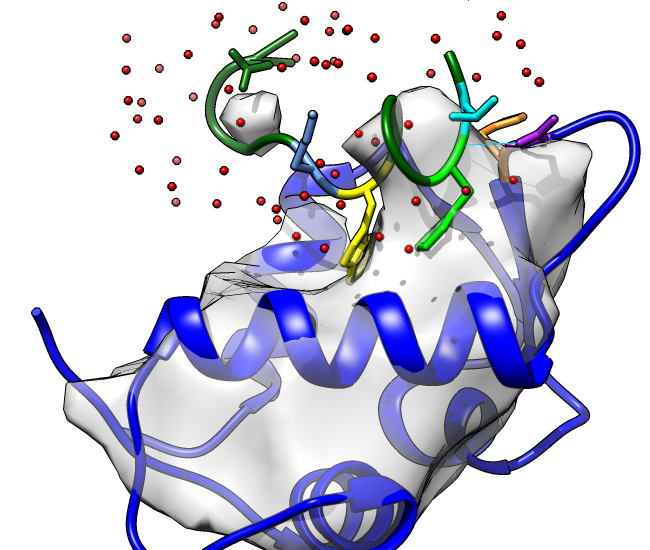
\includegraphics[width=6.5in,height=3.75694in]{media/image4.emf}

\textbf{Figure 4. De-wetting in a protein binding trajectory.} Solvent
features projected onto a 2D tICA subspace corresponding to the first
and second components, tIC\textsubscript{1} and tIC\textsubscript{2}.~
Each color-coded snapshot represents a transition state containing its
own unique molmap (Gaussian smoothing at the 0.015 level) characterizing
instantaneous solvent density. MDM2 (blue): Q71 (purple), H72 (orange)
and p53 (green): L24 (light blue), T18 (red), F19 (pink) and W23 (cyan).

Water traces are displayed below for T18 and W23 of p53, which have been
deemed important residues. Specifically, the 2\textsuperscript{nd}
shells of each are regarded significant, where the trace of water counts
along the trajectory overlaid in Figure 4. demonstrates the transition
from (b) to (c). In addition, the water traces provide insight for the
next transition, (c) to (d).

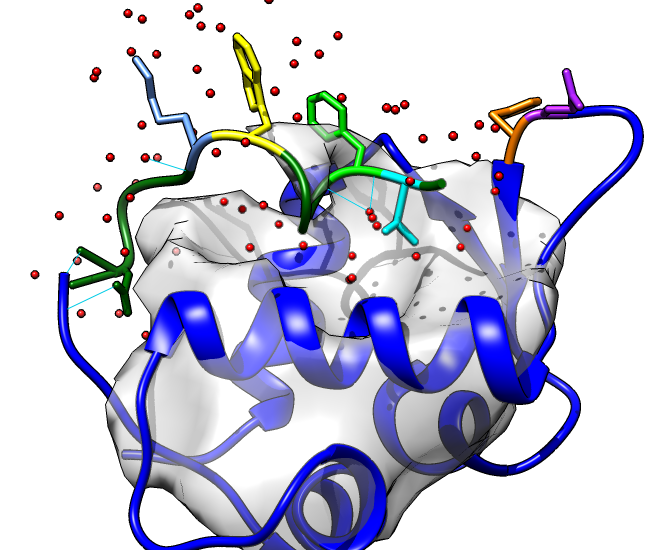
\includegraphics[width=6.5in,height=2.50347in]{media/image5.tiff}

\textbf{Figure 5}. Water counts for W23 and T18 of p53 TAD,
corresponding to the trajectories shown in Figure 4. Changes in. these
observables discernibly follow the movements associated with transitions
(b)-(d).

The hydrogen bond acceptor from the oxygen atom in water molecules is in
fact a primary mechanism of folding. Here, it is found that threonine,
T18 of p53 is found to create hydrogen bonds with water and is shifted
in many of the observed motions. T18 was identified to contain
significant solvent dynamics around 3-6Å. In between residues water acts
as an intermediate state stabilizer in that hydrogen bonds are formed
with the hydroxyl group of polar residues like T18 and Lysine, K24 to
facilitate the structural transformation of the p53 alpha helix.

Instantaneous solvent density from specific movies (posted on website or
supplemental information) suggests the hydrophobic effect plays a key
role in water dynamics. Water are found during important motions of
helix formation and can be found looking for surface cavities.
Scattering of water leads to reorganization to increase polar
interactions and position themselves to a more favorable location. It is
well known that water can become trapped as a result of protein folding.

Many transitions were found that during the binding of p53-MDM2 water
would become trapped inside the hydrophobic pocket. Entrapped waters
don't usually vacate until bulky nonpolar residues such as W23 and F19
of p53 come together and create a greasy surrounding making the waters
uncomfortable, so water molecules slip out creating tunnels or cavities
within the solvent occupancy surface. Another example is located around
T18 of p53 and Q72 of MDM2, where the back-and-forth jostling of water
clusters between these two residues ultimately assists in stability of
the alpha helix. On the contrary, Q72's polarity can be a nuisance for
the helix formation in the vicinity of T18, and may contribute to the
